%%%%%%%%%%%%%%%%%%%%%%% file template.tex %%%%%%%%%%%%%%%%%%%%%%%%%
%
% This is a general template file for the LaTeX package SVJour3
% for Springer journals.          Springer Heidelberg 2010/09/16
%
% Copy it to a new file with a new name and use it as the basis
% for your article. Delete % signs as needed.
%
% This template includes a few options for different layouts and
% content for various journals. Please consult a previous issue of
% your journal as needed.
%
%%%%%%%%%%%%%%%%%%%%%%%%%%%%%%%%%%%%%%%%%%%%%%%%%%%%%%%%%%%%%%%%%%%
%
% First comes an example EPS file -- just ignore it and
% proceed on the \documentclass line
% your LaTeX will extract the file if required
\begin{filecontents*}{example.eps}
%!PS-Adobe-3.0 EPSF-3.0
%%BoundingBox: 19 19 221 221
%%CreationDate: Mon Sep 29 1997
%%Creator: programmed by hand (JK)
%%EndComments
gsave
newpath
  20 20 moveto
  20 220 lineto
  220 220 lineto
  220 20 lineto
closepath
2 setlinewidth
gsave
  .4 setgray fill
grestore
stroke
grestore
\end{filecontents*}
%
\RequirePackage{fix-cm}
%
\documentclass{svjour3}                     % onecolumn (standard format)
%\documentclass[smallcondensed]{svjour3}     % onecolumn (ditto)
%\documentclass[smallextended]{svjour3}       % onecolumn (second format)
%\documentclass[twocolumn]{svjour3}          % twocolumn
%
\smartqed  % flush right qed marks, e.g. at end of proof
%
\usepackage{mhsetup}
\usepackage{amsmath}
\usepackage{mathtools}
\usepackage{natbib}
\usepackage{graphicx}
\usepackage{float}
\usepackage{qtree}
\usepackage[utf8]{inputenc}
\usepackage{gb4e}
\usepackage[T1]{fontenc}
\usepackage{ tipa }
\usepackage{hyperref}
\bibpunct{(}{)}{,}{a}{}{,}
\newcommand{\noteme}[1]{\noindent \textbf{[[JCW:  #1 ]]}}
\renewcommand{\theequation}{\Alph{equation}}

% Insert the name of "your journal" with
\journalname{Journal of }

\begin{document}

\title{Extraposition is Disapppearing
\thanks{digs, geneva, ucl}}
%\subtitle{Do you have a subtitle?\\ If so, write it here}

%\titlerunning{Short form of title}        % if too long for running head

\author{Joel C. Wallenberg}

%\authorrunning{Short form of author list} % if too long for running head

\institute{Joel C. Wallenberg \at
              Newcastle University \\
              Tel.: +44-(0)191-222-7366\\
              \email{joel.wallenberg@ncl.ac.uk}
}

\date{Received: date / Accepted: date}
% The correct dates will be entered by the editor


\maketitle

\begin{abstract}
stuff
\keywords{syntax \and language change \and Indo-European \and evolutionary dynamics \and treebanks}
% \PACS{PACS code1 \and PACS code2 \and more}
% \subclass{MSC code1 \and MSC code2 \and more}
\end{abstract}

\section{Introduction}
\label{intro}
%Kiparsky 1995, Hopper (Hooper?) & Traugott 200?
This squib presents presents important preliminary results demonstrating the existence of a syntactic change which is many times slower than any other that has previously been reported: the syntactic process of relative clause extraposition is being lost in both Germanic and Romance languages.
%Depending on what is driving the change, it may also be a new class of syntactic change. 
As the results are still preliminary and much of their analysis is still unclear, the main goal of this article is to carefully describe a type of syntactic change which presents problems for both synchronic syntactic theory and the theory of language change, but not to present a comprehensive analysis of every aspect of this change at the present time.
Furthermore, this decline in extraposition has been underway for over a thousand years, and while it is nearing completion in modern Portuguese, the change appears to still be ongoing at the present time. That is to say, the construction in (\ref{construct2}) is currently in decline, and likely on its way to extinction:

\begin{exe}
    \ex %English (constructed):
    \begin{xlist}
         \ex \label{construct1} Someone who you like is coming to the party.
         \ex \label{construct2} Someone is coming to the party who you like.
        \end{xlist}
\end{exe}


This clear result has the following consequence: any analysis of relative clauses (and extraposition) must take into account the fact that the extraposed and \textsl{in situ} variants are, in some sense, ``competing grammars'' \citep[in the sense of][inter alia]{kroch1989, kroch1994}; they must be in competition in language use, as one variant is in the process of replacing the other.
The fact that such slow changes exist, and that their effects on synchronic language use can be demonstrated, should cause all researchers in synchronic syntax to question whether all purported cases of ``optional'' movements are in fact changes in progress.
Perhaps ``optional'' has no coherent meaning in grammar, outside of the meaning of change in progress.

The paper is organised as follows.
First, I report quantative data that relative clause extraposition is being lost in the following languages: English, Icelandic, French, and Portuguese, using seven different parsed diachronic corpora (i.e. treebanks).
Next, I discuss the idea that the extraposed and \textsl{in situ} variants are ``competing grammars'', syntactic variants which are mutually exclusive and competing in language use, and suggest some consequences this has for the analysis of relative clauses.
In section \ref{slow}, I discuss the fact that the extraposed variant is specialized for particularly heavy relative clauses, which is the factor that slows the change down to a degree that it is only observable over a period of a thousand years.
Finally, section \ref{pie} builds on \ref{kiparsky1995} and presents the possibility that this change began back in pre-history, at a time when true relative clauses were first innovated in Romance and Germanic, and has been underway ever since that time.



\section{Decline in Relative Clause Extraposition}
\label{relclause}

The data in \ref{results} below show a remarkably slow decline in the frequency of relative clause extraposition from subject DPs in four languages: English, Icelandic, French, and Portuguese. I originally collected this data to test the hypothesis that the frequency of relative clause extraposition was stable over time in a number of languages; as you will see below, though the change is slow enough to be unobservable without data from over a period of many hundreds of years, that hypothesis can be soundly rejected.

\subsection{Methods}

It is worth noting that the type of data presented below is entirely unobtainable without diachronic parsed corpora (i.e. treebanks), which have been annotated at a very high level of accuracy (i.e. they have been hand-corrected by expert syntacticians, not only automatically parsed). For this study, the following parsed diachronic corpora were used: for English, the \textsl{York-Toronto-Helsinki Corpus of Old English Prose (YCOE)} \citep{ycoe}, the \textsl{Penn-Helsinki Parsed Corpus of Middle English 2 (PPCME2)} \citep{ppcme2}, the \textsl{Penn-Helsinki Parsed Corpus of Early Modern English (PPCEME)} \citep{ppceme}, and the \textsl{Penn Parsed Corpus of Modern British English (PPCMBE)} \citep{ppcmbe}; for Icelandic, the \textsl{Icelandic Parsed Historical Corpus (IcePaHC)} \citep{icepahc09}; for Old and Middle French, the \textsl{MCVF Corpus} \citep{mcvf}; and for historical Portuguese, the \textsl{Tycho Brahe Corpus of Historical Portuguese} \citep{tychobrahe}.

Finite clauses containing a relative clause modifying a subject or object were extracted from the corpora using CorpusSearch coding queries \citep{corpussearch}, and coded for the following variables: the response variable of whether or not the relative clause was extraposed, whether it modified a subject or object DP, its weight in number of words, whether the clause occurred in reported speech or not, and the date of the text the clause appeared in.\footnote{If no precise date of composition was available, as was the case for many Old English and Old Icelandic texts, we used an estimated date of composition wherever possible, or a manuscript date in cases where there is no clear consensus on the date of composition. In all cases, we follow the dates provided by the documentation of the diachronic corpora, following the philological sources they cite.} These variables were controlled for in all subsequent statistical analysis.

%åFor English, Icelandic, and Portuguese, only prose texts are 

All coding queries and the extracted datasets are available at in the following public \textsl{git} directory: \url{github.com/joelcw/tyneside/tree/master/extraposition/queriesandoutput}.
%were coded so that the effects of these variables could be controlled for in statistical analysis.



%agnostic as the rightward/leftward-movement question
%Cite Anton about phonological weight being continuous, not discrete !!!


%extraposition in modern Dutch and German, which has specialized along a grammatical, categorical dimension

\subsection{Results}
\label{results}

For the four languages I investigated, English, Icelandic, French, and Portuguese, there is a slow but steady decline in the rate of relative clause extraposition over the course of each language's written history (given the corpora we currently have), compared to the use of \textsl{in situ} relative clauses. This is shown in Figures \ref{engfig}-\ref{portfig}. (Raw numbers by century are provided in the Appendix; for extracted data sets in the form of lists of codes, please see files ending in ``.ooo'' in the github directory linked above, i.e. \url{github.com/joelcw/tyneside/tree/master/extraposition/queriesandoutput/*.ooo}.) \noteme{Do I need this last?}

\begin{figure}

  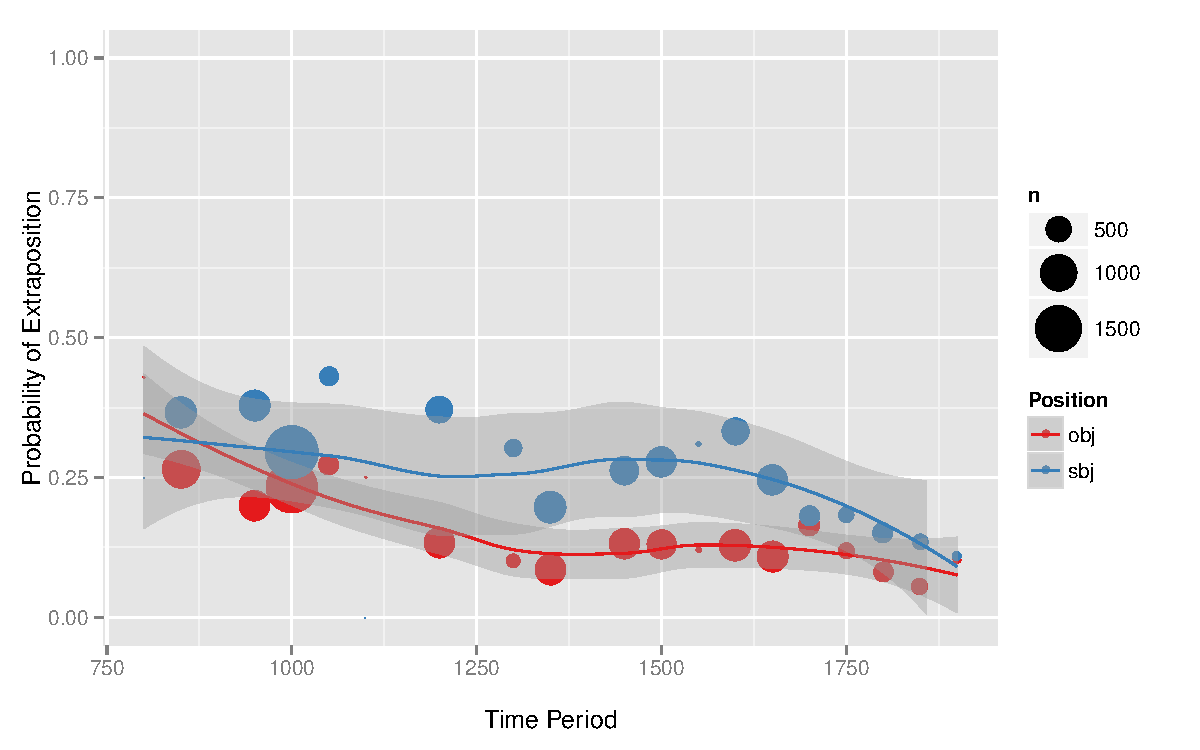
\includegraphics[width=1.1\textwidth]{stableVarTalks/exSbjObjYearBinned50Loessymeb.pdf}
\caption{Declining proportion of relative clause extraposition (vs. \textsl{in situ}), from early Old English prose through modern English. N = 18530 relative clauses.}
\label{engfig}       % Give a unique label
\end{figure}

\begin{figure}

  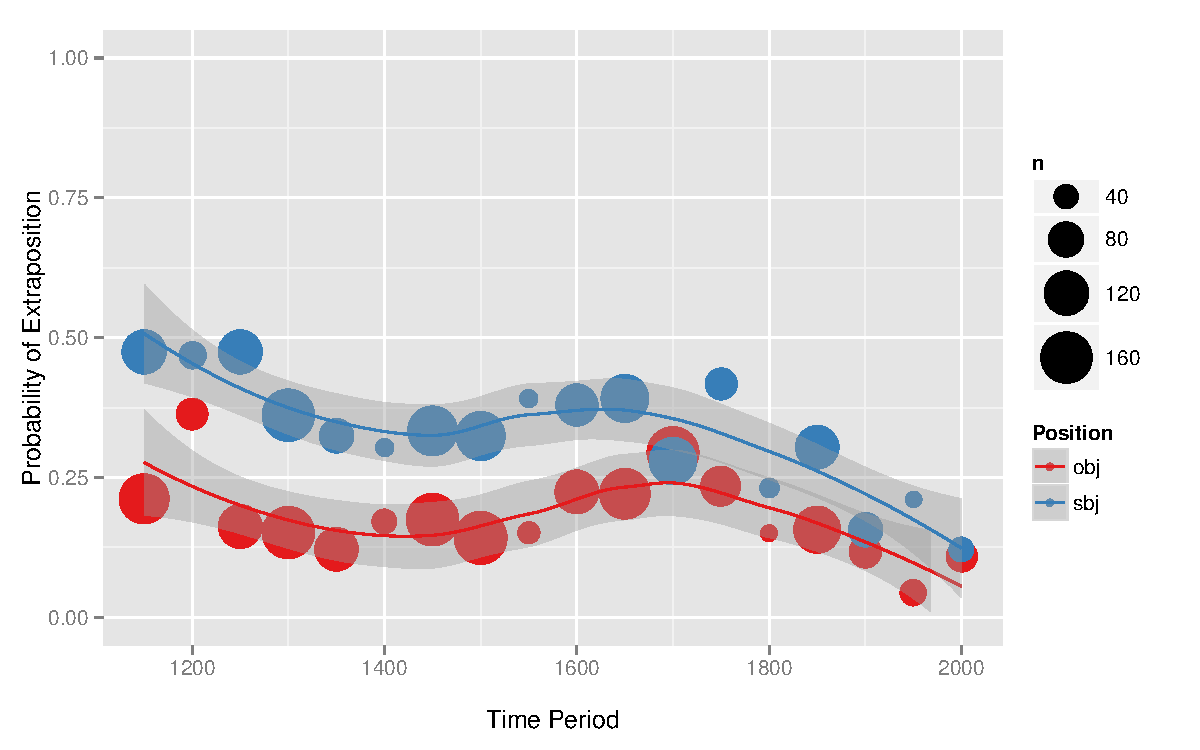
\includegraphics[width=1.1\textwidth]{stableVarTalks/exSbjObjYearBinned50Loessice.pdf}
\caption{Declining proportion of relative clause extraposition (vs. \textsl{in situ}) from subject and object positions, early Old Icelandic prose through modern Icelandic. N = 3486 relative clauses.}
\label{icefig}       
\end{figure}

\begin{figure}
  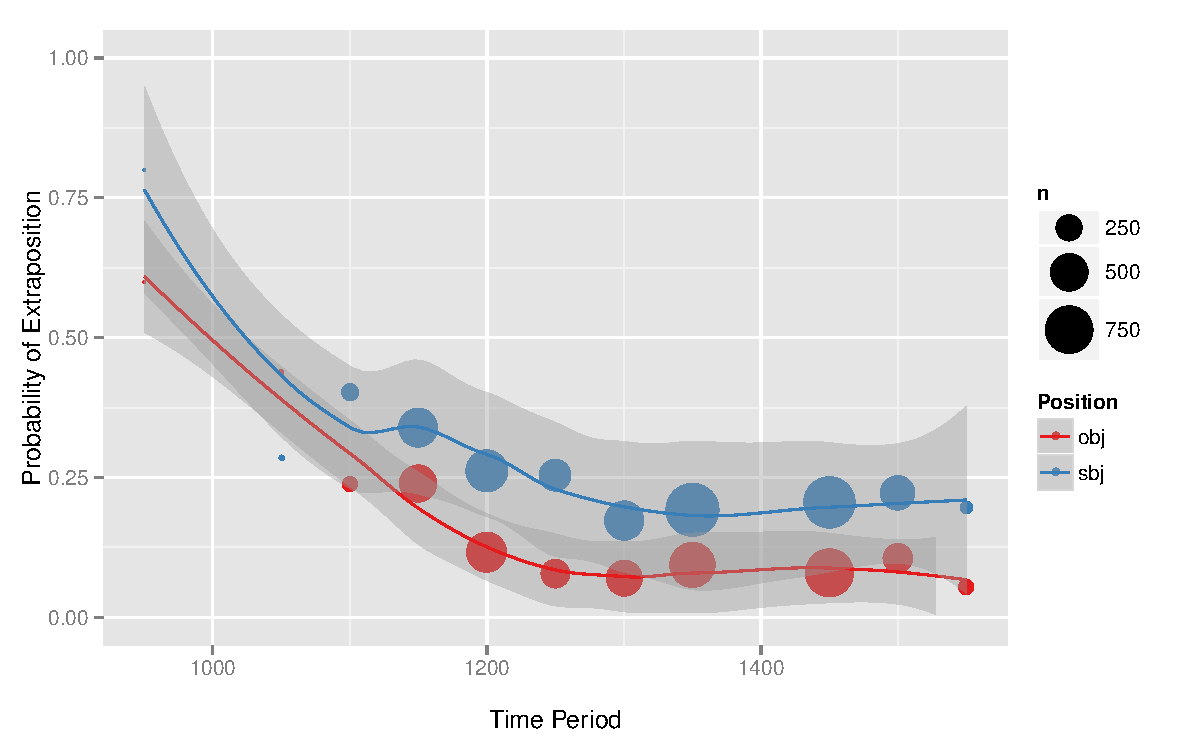
\includegraphics[width=1.1\textwidth]{stableVarTalks/exSbjObjYearBinned50Loessfre.pdf}
\caption{Declining proportion of relative clause extraposition (vs. \textsl{in situ}) from subject and object positions, Old and Middle French. N = 8207 relative clauses.}
\label{frefig}       
\end{figure}

\begin{figure}
  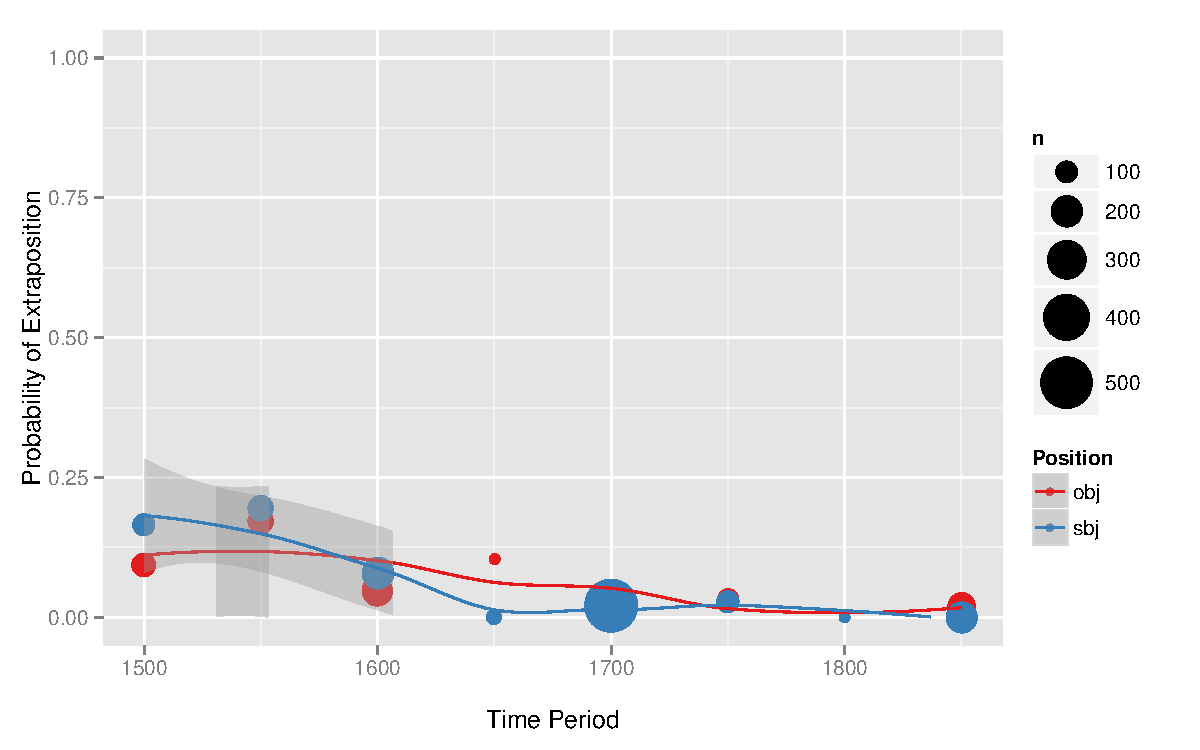
\includegraphics[width=1.1\textwidth]{stableVarTalks/exSbjObjYearBinned50Loessport.pdf}
\caption{Declining proportion of relative clause extraposition (vs. \textsl{in situ}) from subject and object positions, 15th-19th c. Portuguese. N = 2398 relative clauses.}
\label{frefig}       
\end{figure}



As can be seen in the Figures for English (Figure \ref{engfig}) and Icelandic (Figure \ref{icefig}), the decline in extraposition is so slow that it could have been easily missed if the corpora of English (collectively) and Icelandic were not at sufficient time-depth (over 1000 years of data for each); any time-window of only a few hundred years would likely be too small to detect such a change at all.

For comparison, I conducted the same study on the Parsed Corpus of Early English Correspondence \citep[PCEEC][]{pceec}, which covers a period from the 15th through 17th centuries. The results of that study make the frequency of extraposition appear to be stable over time, shown in Figure \ref{pceecfig}.

\begin{figure}
  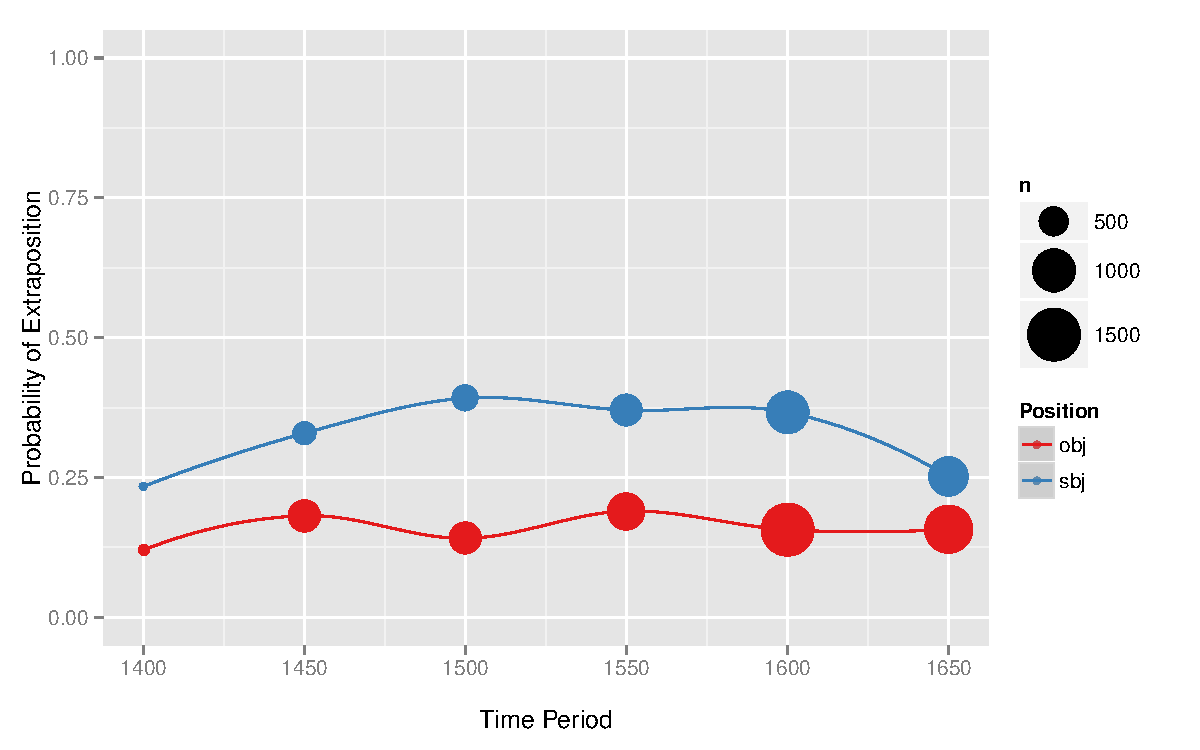
\includegraphics[width=1.1\textwidth]{stableVarTalks/exSbjObjYearBinned50.pdf}
\caption{Declining proportion of relative clause extraposition (vs. \textsl{in situ}) from subject and object positions, Parsed Corpus of Early English Correspondence. N = 8073 relative clauses.}
\label{pceecfig}       
\end{figure}

\noindent The results in Figure \ref{pceecfig} match the results from the larger English corpora for the same time period (compare Figure \ref{engfig}), but miss the change entirely; simply by accident, the 250-year time-slice of the PCEEC happens to not reflect the change, which then becomes visible once we observe a larger diachronic window.

Nevertheless, fitting a logistic regression model shows that the decline in extraposition is statistically significant in each of the languages; an interaction between text year and extraposition significantly improves model fit (p < 0.00001 for all languages), controlling for all other interactions involving: matrix/subordinate clause-type, simple text vs. reported speech, subject vs. object position, and weight of the subordinate clause (i.e. length measured in number of words).

Interestingly, a model constrained to have the same slope parameter for the decline in both Icelandic and English (controlling for the same factors above) fits well, and not significantly better than a model which allows different slope terms for the two languages (p $\approx$ 0.45). This is reminiscent of the Constant Rate Effect \citep[][among others]{kroch1989, pintzuk1991, santorini1993a}, which states the different surface realizations of the same underlying linguistic object will change with the same slope as each other as that underlying linguistic object changes. Though the situation here is not one of comparing different linguistic contexts, but rather different populations of speakers (i.e. Icelandic and English), perhaps the same basic logic applies: the same trajectory of change could indicate that the same forces are underlying the change in both populations, both in terms of what is driving the change, and in terms of which basic linguistic object is undergoing change. 

However, any model with includes the French and Portuguese data fits significantly worse when it assumes the same slope for the change over time. This is true if French and Portuguese are modelled together, separately from Icelandic and English, or if any combination of languages including either French or Portuguese are modelled together. This either means that these languages show a similar-looking, but ultimately different change (at least at the time points we are observing), or that some other feature of those data sets is obscuring what should be the same slope as in Icelandic and English. Since the text-sampling methods were designed to control for genre effects over time in the Icelandic and English corpora, but this was not done in the same way for the Tycho Brahe and MCVF corpora (and the latter is the only corpus which contains significant amounts of poetry as well as prose), we cannot rule out the possibility that the estimated slopes for French and Portuguese have been obscured by factors that are extraneous to the issue under investigation.

%, and genre (for IcePaHC only\footnote{Genre is easier to code for in the IcePaHC annotation. }



\section{Extraposition As Competing Grammars}

unstable
It means that in all four languages (with the possible exception of modern Portuguese), even though the loss of extraposition began at least a thousand years ago, the change is still in progress at the present time. Thus, the seeming optionality between extraposed and non-extraposed relative clauses is really most simply described as the code-switching that is characteristic of a change in progress, as established

\section{Why So Slow?}
\label{slow}

\section{Origin of Relative Clauses}
\label{pie}

%continued presence of CP-CARs, compare to Vedic in Kiparsky



%Cite other paper with Joe

\section{Conclusions}












%
% For two-column wide figures use
%\begin{figure*}
% Use the relevant command to insert your figure file.
% For example, with the graphicx package use
%  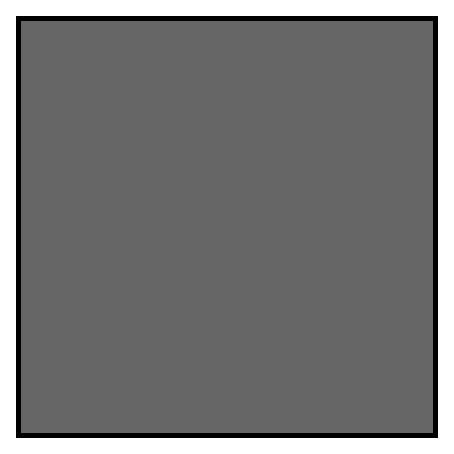
\includegraphics[width=0.75\textwidth]{example.eps}
% figure caption is below the figure
%\caption{Please write your figure caption here}
%\label{fig:2}       % Give a unique label
%\end{figure*}
%
% For tables use
%\begin{table}
% table caption is above the table
%\caption{Please write your table caption here}
%\label{tab:1}       % Give a unique label
% For LaTeX tables use
%\begin{tabular}{lll}
%\hline\noalign{\smallskip}
%first & second & third  \\
%\noalign{\smallskip}\hline\noalign{\smallskip}
%number & number & number \\
%number & number & number \\
%\noalign{\smallskip}\hline
%\end{tabular}
%\end{table}


%\begin{acknowledgements}

%\end{acknowledgements}

% BibTeX users please use one of
%\bibliographystyle{spbasic}      % basic style, author-year citations
%\bibliographystyle{spmpsci}      % mathematics and physical sciences
%\bibliographystyle{spphys}       % APS-like style for physics
\bibliographystyle{linquiry2} %use spbasic for journal of comparative gmc linguistics, etc.
\bibliography{joelrefs}   % name your BibTeX data base

\section*{Appendix}

\end{document}
% end of file template.tex

 